\documentclass[tikz,border=2pt]{standalone}
\usepackage{amsmath,amssymb}
\usepackage{tikz}

\begin{document}
% An equivalence relation chops a set into disjoint classes: here the integers 0..8 under
% "same remainder modulo 3".
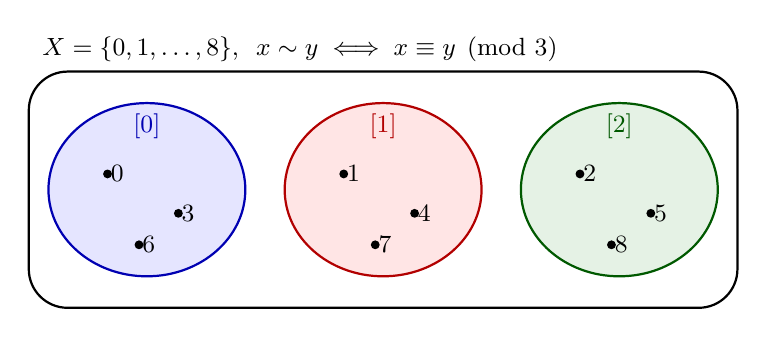
\begin{tikzpicture}[every node/.style={font=\small}]
	\draw[thick, rounded corners=14pt] (-0.9,-1.0) rectangle (8.1,2.0);
	\node[anchor=south west] at (-0.85,2.0) {$X=\{0,1,\dots,8\}$, $\ x\sim y\iff x\equiv y\pmod 3$};
	\foreach \c/\x/\col in {0/0.6/blue, 1/3.6/red, 2/6.6/green!50!black} {
		\fill[\col!10] (\x,0.5) ellipse (1.25 and 1.1);
		\draw[\col!70!black, thick] (\x,0.5) ellipse (1.25 and 1.1);
		\node[\col!70!black, font=\small] at (\x,1.3) {$[\c]$};
	}
	\foreach \v/\x/\y in {0/0.1/0.7, 3/1.0/0.2, 6/0.5/-0.2, 1/3.1/0.7, 4/4.0/0.2, 7/3.5/-0.2, 2/6.1/0.7, 5/7.0/0.2, 8/6.5/-0.2} {
		\fill (\x,\y) circle (1.6pt);
		\node[right, font=\small, inner sep=1pt] at (\x,\y) {$\v$};
	}
\end{tikzpicture}
\end{document}
